\chapter[Testing]{Testing}
\label{cap:preliminares.testing}

Garantizar que un programa realiza de manera correcta las tareas para las cuales fue desarrollado se encuentra dentro de los problemas m\'as desafiantes y uno de los m\'as importantes temas de investigaci\'on en el contexto de la Ingenier\'ia de Software \cite{bibliography.books.GhezziBook,bibliography.books.PressmanBook,DBLP:series/txcs/Jalote05}. Es un tema central en la calidad de software, que demanda una cantidad significativa de recursos \cite{bibliography.books.JaloteBook}, y por lo tanto tiene impacto sustancial en el costo de producci\'on de software. 

La introducci\'on de defectos puede ocurrir en cualquier etapa del desarrollo del software. El costo de resolver los problemas asociados a corregir estas deficiencias, sin embargo, cambia sutancialmente de acuerdo a la etapa en la cual fue introducido y cu\'ando fue detectado: detectar un error introducido en la etapa de requisitos (por ejemplo, comprensi\'on err\'onea de alg\'un aspecto del problema a resolver) en la etapa de testing puede costar hasta 100 veces m\'as que hacerlo durante la etapa de requisitos, donde fue introducido \cite{bibliography.books.JaloteBook}. De la misma manera, las t\'ecnicas para la detecci\'on de defectos de software cambian, de acuerdo al tipo de defecto, y a la etapa del proceso de desarrollo en la que se aplican. El \emph{testing}, que en esencia consiste en ejecutar un programa bajo un conjunto espec\'ifico de escenarios, contrastando el comportamiento actual con el esperado \cite{bibliography.books.AmmannOffutt}, es el enfoque m\'as com\'unmente usado para la detecci\'on de defectos de software, que dada su naturaleza, se aplica luego de la implementaci\'on de la funcionalidad a evaluar. A pesar de sus conocidas limitaciones, que E.~W.~Dijkstra resumi\'o notablemente en su conocida frase \emph{``Program testing can be used to show the presence of bugs, but never to show their absence!''} \cite{Dijkstra:1972:CIN:1243380.1243381}, testing es la t\'ecnica de mayor aplicaci\'on, en la pr\'actica, para brindar garant\'ias (parciales) de calidad de software. La limitaci\'on central del testing est\'a asociada al hecho de que en general es inviable, o imposible, ejecutar de manera exhaustiva un programa bajo todos sus posibles escenarios de ejecuci\'on (es decir, considerando todas sus entradas, directas e indirectas). Por esta raz\'on, es necesario seleccionar una muestra, un subconjunto de todos los escenarios posibles, sobre los cuales se realizar\'a la evaluaci\'on del comportamiento del software. Claramente, el testing, como t\'ecnica de verificaci\'on, es una t\'ecnica necesariamente incompleta, aunque goza de una simplicidad y escalabilidad que otros enfoques de verificaci\'on, especialmente aquellos basados en an\'alisis est\'atico, tienen dificultades de alcanzar.

Un \emph{test} consta b\'asicamente de los siguientes pasos: 
\begin{enumerate}
	\item Preparaci\'on (\emph{Arrange}), define los datos necesarios para el escenario bajo el cual se va a ejecutar el test. A modo de ejemplo, consideremos el test de la Figura~\ref{figures.examples.test.manual}. La primera l\'inea de este test, en la cual se define el escenario sobre el cual se va a evaluar la implementaci\'on de una calculadora, corresponde al \emph{arrange}.
	
	\item Ejecuci\'on (\emph{Act}), es la ejecuci\'on del programa a evaluar. Generalmente incluye la obtenci\'on del resultado de dicha ejecuci\'on, para su posterior contrastaci\'on con el resultado esperado. La l\'inea 2 de la Figura~\ref{figures.examples.test.manual} ejecuta una funcionalidad de la calculadora, a trav\'es del m\'etodo \texttt{Calculator\#evaluate(String)}, para la expresi\'on definida en el arrange; esta l\'inea corresponde al \emph{act} del test. 
	
	\item Evaluaci\'on (\emph{Assert}), consiste en la verificaci\'on de que el resultado obtenido, ya sea un valor de salida o un estado del programa, se corresponde con el esperado. La \'ultima l\'inea de la Figura~\ref{figures.examples.test.manual} eval\'ua que la ejecuci\'on del m\'etodo \texttt{Calculator\#evaluate(String)}, para la expresi\'on definida en el arrange, da como resultado \texttt{16}; esta l\'inea corresponde al \emph{assert} del test.
\end{enumerate}

\begin{figure}
	\begin{lstlisting}[frame=single, mathescape=true,numbers=left,framexleftmargin=1.5em,basicstyle={},xleftmargin=.055\textwidth,xrightmargin=.01\textwidth]
 la entrada a evaluar es "(1 + 3)^2"
 evaluar Calculator#evaluate con la entrada anterior
 el resultado obtenido debe ser 16
	\end{lstlisting}
	\caption{Ejemplo de un test}
	\label{figures.examples.test.manual}
\end{figure}

Evidentemente, c\'omo se elige la muestra de entradas que ser\'a utilizada para testing afecta significativamente la habilidad del proceso de testing en la detecci\'on de fallas en el software. Recordemos que el programa bajo an\'alisis se evaluar\'a sobre un conjunto de entradas, con la intenci\'on de verificar que el comportamiento real del software coincide con el esperado en estos casos, y a partir de este resultado ``generalizar'' el resultado a todos los posibles escenarios de ejecuci\'on. Dado que la selecci\'on de los escenarios para testing es crucial para este proceso, se necesita alg\'un tipo de criterio, denominado criterio de testing, que asista en la selecci\'on de los escenarios. Los criterios de testing ayudan a seleccionar escenarios, y al mismo tiempo sirven como \emph{m\'etricas} de la calidad de conjuntos de tests. 

Los criterios de testing t\'ipicamente se clasifican en \emph{caja blanca} (white box), si tienen en cuenta la estructura del c\'odigo bajo an\'alisis, o \emph{caja negra} (black box), si en cambio se concentran en la especificaci\'on del programa bajo prueba. Los criterios de testing, independientemente de la clase a la que pertenezcan, definen, directa o indirectamente, una m\'etrica, que permite evaluar la calidad de una test suite. Esta medida se puede entender como una m\'etrica de cu\'an exhaustivamente eval\'ua una test suite el comportamiento del software, o equivalentemente, cu\'an probable es que existan defectos en el software, que pasen desapercibidos a la suite. Las medidas son, por supuesto, indirectas. 

\section{Automatizaci\'on de la Ejecuci\'on de Tests}
\label{sec:preliminares.testing.automation}

Si bien la definici\'on de test dada anteriormente no menciona ejecutabilidad, sino que simplemente se limita a describir los pasos o etapas que constituyen un test, es directo suponer que estos pasos son, con excepci\'on quiz\'as del \emph{assert}, evidentemente implementables. Decimos que la implementaci\'on de la etapa de \emph{assert} es menos evidente porque este paso es en muchos casos, cuando se llevan adelante procesos ad hoc de testing, realizado manualmente: es el desarrollador o usuario quien contrasta el resultado real con el resultado esperado. Sin embargo, muchas caracter\'isticas del resultado esperado de un programa son, en muchos casos, verificables de manera directa, y por lo tanto tambi\'en lo es su automatizaci\'on. 

Existen numerosas bibliotecas disponibles para automatizar el proceso de ejecuci\'on de tests. Una de estas, que goza de enorme popularidad, es la biblioteca \emph{JUnit}, para tests de unidad en Java. En la Figura~\ref{figures.examples.test.junit} se muestra el ejemplo anterior implementado en \emph{Java} utilizando la biblioteca \emph{JUnit}.

\begin{figure}[ht!]
	\begin{lstlisting}[frame=single, mathescape=true,numbers=left,framexleftmargin=1.5em,language=Java,basicstyle={},xleftmargin=.055\textwidth,xrightmargin=.01\textwidth]
  String expression = "(1 + 3)^2";
  Integer result = calculator.evaluate(expression);
  assertEquals(new Integer(16),result);
	\end{lstlisting}
	\caption{Ejemplo de un test JUnit}
	\label{figures.examples.test.junit}
\end{figure}

\subsection{Generaci\'on autom\'atica de escenarios de testing}

La automatizaci\'on de la ejecuci\'on de los tests es muy \'util, por diversas razones, pero esencialmente porque permite ejecutar y re-ejecutar los tests asociados a una aplicaci\'on de manera muy conveniente y eficientemente, especialmente cuando la comprobaci\'on de que los resultados esperados coinciden con los obtenidos (los \emph{asserts}) tambi\'en se chequean autom\'aticamente. Sin embargo, la construcci\'on de tests es un proceso cuya automatizaci\'on es sustancialmente m\'as dif\'icil, entre otras razones porque requiere que alguien provea los escenarios en los cuales evaluar un programa particular. La generaci\'on de escenarios de prueba de manera autom\'atica tiene gran valor pr\'actico, puesto que permite automatizar parte del proceso de \emph{generaci\'on} de tests, y reducir los costos asociados a este proceso. 

Actualmente existen numerosas aplicaciones cuyo objetivo principal es la generaci\'on autom\'atica de entradas para testing. Algunos de los enfoques utilizados para la generaci\'on autom\'atica de entradas incluyen:
\begin{itemize}
\item \emph{Generaci\'on aleatoria de entradas}, que consiste en elegir, para alg\'un conjunto de valores predefinidos y de manera aleatoria, elementos del mismo para usar como entradas del programa a evaluar. Esta metodolog\'ia es muy sencilla de implementar para valores de tipos no estructurados, como por ejemplo enteros y valores num\'ericos. Para la generaci\'on de valores de tipos estructurados, como por ejemplo una lista simplemente encadenada, es necesario combinar la generaci\'on aleatoria para cada componente que conforma el tipo estructurado. Sin embargo, estos tipos estructurados tienen invariantes que deben ser satisfechos para que una instancia (un valor de este tipo) sea considerada v\'alida. En las Figuras \ref{figures.examples.testing.random.primitive} y \ref{figures.examples.testing.random.structure} se pueden ver ejemplos de generaci\'on aleatoria para tipos primitivos y estructurados respectivamente. %Un detalle a tener en cuenta en el ejemplo de generaci\'on aleatoria para tipos estructurados, es que la construcci\'on se hace mediante m\'etodos provistos por la misma estructura, en particular, el m\'etodo \lstinline|List#add(int)|. Una alternativa com\'unmente utilizada es generar de menor a mayor complejidad los componentes de las estructuras

\item \emph{Generaci\'on exhaustiva (acotada) de entradas}, que consiste en utilizar todos los valores disponibles dentro de un espacio acotado de entradas del programa a evaluar. Para valores primitivos esto consistir\'ia en utilizar todos los valores entre un valor m\'inimo y un m\'aximo (que definen un dominio acotado). Evidentemente, una cota debe definir un sub-dominio finito, para que la generaci\'on exhaustiva acotada termine. Para valores que corresponden a tipos estructurados, la metodolog\'ia es similar a generaci\'on aleatoria. Esta metodolog\'ia parecer\'ia en primera instancia generar una mayor confianza ya que permite evaluar un programa bajo todas las posibles entradas dentro de una determinada cota. La cantidad de entradas que se obtienen por generaci\'on exhaustiva llegan muy r\'apido a cantidades que hacen al proceso de generaci\'on o al de testing inviable. En \cite{bibliography.testing.generation.KoratBoyapatiKM02} se presenta una herramienta de generaci\'on exhaustiva acotada de instancias para tipos estructurados, y se muestra c\'omo la cantidad de valores generados aumenta exponencialmente respecto a las cotas utilizadas.
\end{itemize}

\begin{figure}
	\small
	\begin{lstlisting}[frame=single, mathescape=true,language=Java,basicstyle={},xleftmargin=.04\textwidth,xrightmargin=.04\textwidth]
  Set intInputs = new Set();
  for (int i = 0; i<10; i++) {
    int rndValue = 10 + random.nextInt(11);
    intInputs.add(rndValue);
  }
	\end{lstlisting}
	\caption[Generaci\'on aleatoria de valores enteros]{Ejemplo de generaci\'on aleatoria de 10 valores enteros entre 10 y 20}
	\label{figures.examples.testing.random.primitive}
\end{figure}

\begin{figure}
	\small
	\begin{lstlisting}[frame=single, mathescape=true,language=Java,basicstyle={},xleftmargin=.04\textwidth,xrightmargin=.04\textwidth]
  Set structuredInputs = new Set();
  for (int i = 0; i<10; i++) {
    int rndSize = random.nextInt(10);
    List rndList = new List();
    for (int elemIdx = 0; elemIdx < rndSize; elemIdx++) {
      int rndValue = random.nextInt(50);
      rndList.add(rndValue);
    }
    structuredInputs.add(rndList);
  }
	\end{lstlisting}
	\caption[Generaci\'on aleatoria de listas]{Ejemplo de generaci\'on aleatoria de 10 listas de enteros con tama\~no entre 0 a 10, y con valores entre 0 a 50}
	\label{figures.examples.testing.random.structure}
\end{figure}

%Ejemplos de herramientas para generaci\'on autom\'atica de escenarios incluyen: \emph{Korat} \cite{bibliography.inputGeneration.korat.BoyapatiKM02} que permite generar entradas estructuralmente complejas dado un conjunto de cotas para los atributos de la estructura y una especificaci\'on mediante un predicado imperativo que indica las estructuras v\'alidas. [AGREGAR]

\subsection{El problema del or\'aculo}

Teniendo la capacidad de generar escenarios de testing de manera autom\'atica, y dado que la ejecuci\'on del programa a evaluar, bajo una entrada particular, es trivial de automatizar, conseguimos automatizar una parte importante de la generaci\'on de tests. Sin embargo, el resultado esperado de la ejecuci\'on de un programa es algo que escapa a la generaci\'on autom\'atica directa, pues depende de la \emph{especificaci\'on} del programa desarrollado. A diferencia de las especificaciones formales al estilo de las provistas en l\'ogica de Hoare o formalismos similares, las especificaciones en los tests suelen ser particulares a cada escenario. Por ejemplo, en el caso del test en la Figura~\ref{figures.examples.test.junit}, el valor esperado \emph{16} es la \emph{especificaci\'on} para ese escenario, y obviamente fue provisto por el desarrollador del test, de manera manual. 

El ejemplo anterior corresponde a un test desarrollado manualmente. En el contexto de la generaci\'on autom\'atica de tests, y con el prop\'osito de automatizar de manera completa la generaci\'on de tests, se necesita entonces alguna fuente de la cual tomar la \emph{especificaci\'on} del comportamiento esperado del software. Este problema, el de dado un programa a evaluar y una entrada espec\'ifica para el mismo poder determinar el resultado esperado de la ejecuci\'on del programa en esa entrada, se conoce como el \emph{problema del or\'aculo}. Existen diferentes enfoques para atacar este problema, entre ellas las siguientes: 
\begin{enumerate}
	\item Describir manualmente la salida esperada. Esta soluci\'on es claramente no autom\'atica, es tediosa e insume tiempo, dado que los resultados esperados se describen por cada test.
	
    \item Provisi\'on de especificaciones del comportamiento esperado. Si se cuenta con una especificaci\'on al estilo de una post-condici\'on, \'esta puede actuar como or\'aculo del comportamiento esperado. Ahora bien, si el objetivo es la automatizaci\'on del proceso de generaci\'on autom\'atica de tests, necesitamos que estas especificaciones sean \emph{ejecutables}, es decir, que puede comprobarse autom\'aticamente, dado un estado espec\'ifico de programa, si el mismo satisface la especificaci\'on o no. A modo de ejemplo, si necesitamos producir tests para un m\'etodo que ordena listas de enteros, el resultado deben ser listas que sean permutaciones de la original, y que est\'en ordenadas. Esto se puede comprobar mec\'anicamente, y actuar\'ia como or\'aculo del comportamiento esperado. 
	
	\item Testing diferencial, el cual consiste en, dado un programa bajo evaluaci\'on \texttt{P} y una entrada \texttt{E} sobre la cual se quiere evaluar el comportamiento de \texttt{P}, en la utilizaci\'on de un programa alternativo (ya implementado) \texttt{P$\prime$} con el \emph{mismo} comportamiento que el esperado de \texttt{P}. El or\'aculo constar\'a de un chequeo del estilo de \texttt{P$\prime$(E) == P(E)}. Evidentemente, este enfoque requiere una confianza suficiente en el correcto comportamiento de \texttt{P$\prime$} (que puede ser, por ejemplo, una versi\'on del programa desarrollado m\'as simple y posiblemente menos eficiente, pero cuya correcci\'on es m\'as f\'acil de garantizar). 
	
	\item Testing de regresi\'on, el cual se puede entender como un caso particular de \emph{testing diferencial}, donde una versi\'on anterior del programa a evaluar se utiliza como alternativa ``confiable''. Esta t\'ecnica es utilizada principalmente para evaluar que el comportamiento previo de un programa no fue modificado involuntariamente al, por ejemplo, agregar nuevas caracter\'isticas.
	
\end{enumerate}

\pagebreak
\subsection{Modelo RIP}

La existencia de fallas en el c\'odigo no es, en muchos casos, f\'acil de detectar. El modelo RIP describe, precisamente, las condiciones que deben darse para la detecci\'on de una falla: 
\begin{itemize}
\item \emph{\texttt{R}eachability}, el defecto en el c\'odigo debe ser alcanzable por la ejecuci\'on del programa bajo alg\'un escenario particular;
\item \emph{\texttt{I}nfection}, el defecto debe ``infectar'' el estado del programa, es decir, al ejecutar el c\'odigo que contiene el defecto, debe ocurrir un cambio en el estado del programa que difiere del estado del programa si el mismo no tuviera el defecto (o difiere respecto al estado esperado); 
\item \emph{\texttt{P}ropagation}, el cambio del estado debe propagarse hasta alg\'un punto observable, para permitir diferenciar una salida incorrecta (error) de la correcta.
\end{itemize}

\begin{figure}
	\begin{lstlisting}[frame=single,numbers=left, mathescape=true,framexleftmargin=1.5em,language=Java,basicstyle={},xleftmargin=.055\textwidth,xrightmargin=.01\textwidth]
  public int max(int a, int b) {
    int result = a;
    if (a > b) {
      result = a;
    } else if (b < a) {
      result = b;
    }
    return result;
  }
	\end{lstlisting}
	\caption{Una implementaci\'on incorrecta de un m\'etodo \emph{max}}
	\label{figures.examples.testing.rip}
\end{figure}

La Figura~\ref{figures.examples.testing.rip} contiene una implementaci\'on de un programa que calcula el m\'aximo entre dos n\'umeros. El defecto se encuentra en la segunda condici\'on, \texttt{b < a}. Cualquier entrada en la cual no se cumpla que \texttt{a > b}, va alcanzar la sentencia con el defecto; la infecci\'on se da cuando una entrada que cumpla con \texttt{b > a}, no cambia el valor de \texttt{result} para contener el valor de \texttt{b}; la propagaci\'on se da porque el valor incorrecto en \texttt{result} se retorna en la \'ultima sentencia del programa. Incluso al tener un escenario que cumpla con el modelo \emph{RIP} para un defecto, \'este no va a ser detectado si no se cuenta con un or\'aculo apropiado, en este caso, validar que por ejemplo para los valores \emph{5} y \emph{3}, el resultado esperado es \emph{5}.

\subsection{Criterios de cobertura}
\label{sec:preliminares.testing.covcriteria}

%Queda en evidencia la necesidad de un criterio para evaluar la calidad de un conjunto de tests. Como condici\'on de terminaci\'on para un proceso (ya sea manual o autom\'atico) de generaci\'on de tests, as\'i como para evaluar el conjunto de tests utilizados para poder medir la relaci\'on entre el hecho de que \'estos pasen y la confianza en que el programa bajo evaluaci\'on sea correcto.

Como se mencion\'o anteriormente, al utilizar testing como t\'ecnica para evaluar a un programa con respecto a las tareas que \'este realiza, es necesario seleccionar un conjunto finito de escenarios sobre el cual ejecutar y evaluar el programa. La selecci\'on debe hacerse de forma tal que si el comportamiento del programa es el correcto dentro de los escenarios seleccionados, sea posible generalizar el correcto comportamiento a todos los escenarios posibles. Intuitivamente lo que se busca es poder seleccionar el conjunto de escenarios con la mejor capacidad de detectar potenciales fallas.
Analizar la capacidad de un conjunto de tests en detectar fallas potenciales no es posible, al menos de manera directa, por la raz\'on de que \'estas no son conocidas. En la pr\'actica, la evaluaci\'on de la capacidad de un conjunto de tests en detectar fallas potenciales se realiza de manera indirecta, donde el objetivo es definir una m\'etrica tal que mientras m\'as alto sea el valor asociado a la misma, mayor sea la confianza sobre los tests en detectar fallas potenciales.

Los criterios de cobertura definen m\'etricas de evaluaci\'on generando metas, o requisitos, para la test suite bajo evaluaci\'on, y eval\'uan cu\'antas de estas metas u objetivos son satisfechas por la suite. Un test espec\'ifico puede alcanzar o ``cubrir'' varias metas simult\'aneamente. Dado que un criterio de evaluaci\'on para una test suite no puede directamente analizar la capacidad del mismo en detectar fallas (salvo para aquellas conocidas), en el dise\~no de criterios de testing se intenta construir metas evaluables, y que indirectamente impliquen, o est\'en relacionadas con, la posibilidad de detectar fallas. El modelo \emph{RIP} ayuda al dise\~no de criterios, como veremos a continuaci\'on.

Como criterios de cobertura, aquellos denominados de \emph{caja blanca}, se basan en la estructura del programa para generar metas a cubrir. Por ejemplo, \emph{cobertura de sentencias} genera como metas la ejecuci\'on de las sentencias del programa. Este criterio se enfoca principalmente en \emph{alcanzabilidad} (reachability), claramente influenciado por el modelo RIP: para que una suite sea capaz de detectar defectos, debe en principio alcanzarlos. 

Los criterios de \emph{caja negra} se enfocan en la especificaci\'on del programa para generar metas. Por ejemplo, el criterio de \emph{partici\'on de clases de equivalencia} se enfoca en dividir las entradas en conjuntos para los cuales el comportamiento del programa deber\'ia ser ``similar''. En el caso de \emph{max}, se podr\'ian definir diferentes clases, por ejemplo que el primer valor sea menor que el segundo, que sean iguales, o que el primer valor sea mayor que el segundo. 

A modo de ejemplo para criterios de cobertura de caja blanca, consideremos el c\'odigo que se muestra en la Figura~\ref{figures.code.coverageExample}: el m\'etodo \emph{countEvenIn(int[])} toma como entrada un arreglo de enteros y retorna la cantidad de n\'umeros en el arreglo que son pares. La l\'ogica del programa es bastante simple: se recorre uno a uno los elementos del arreglo y se verifica si el resto de dividir un elemento por 2 es cero; si lo es entonces el elemento es par y se incrementa una variable donde efectivamente se cuenta cu\'antos pares se encontraron. El criterio de cobertura de sentencias genera como objetivos a cubrir la ejecuci\'on de cada sentencia en el programa bajo evaluaci\'on. La \emph{cobertura de ramas} a\~nade como requisitos que las sentencias de bifurcaci\'on (sentencias \emph{if}, \emph{while}, \emph{for}, entre otras) se ejecuten una vez con su condici\'on siendo verdadera y otra con \'esta siendo falsa. Solamente con un test que eval\'ue el m\'etodo con un arreglo de tama\~no 1 conteniendo un n\'umero par, se obtiene una cobertura del 100\% para sentencias (Figura~\ref{figures.examples.coverage.fullCoverage}). Sin embargo, si evaluamos cobertura de ramas podemos observar que con este test no logramos una cobertura del 100\% (Figura~\ref{figures.examples.coverage.stmtCoverage}), en particular porque no se eval\'ua el caso en el cual un elemento es impar. Al generar tests para este criterio podemos simplemente cambiar la entrada a un arreglo de tama\~no 4 con los elementos 1, 2, 3, y 4, obteniendo una cobertura de ramas del 100\% (Figura~\ref{figures.examples.coverage.fullCoverage}).

\begin{figure}
	\lstinputlisting[frame=single,basicstyle=\small, language=Java, tabsize=1,framexleftmargin=.068\textwidth,xleftmargin=.08\textwidth,xrightmargin=.01\textwidth,literate={\ \ }{{\ }}1]{results/draft/CoverageExample.java}
	\caption[M\'etodo \emph{countEvenIn(int[])}]{M\'etodo para contar n\'umeros pares en un arreglo de enteros.}
	\label{figures.code.coverageExample}
\end{figure}

%[frame=single,numbers=left, mathescape=true,framexleftmargin=1.5em,language=Java,basicstyle={},xleftmargin=.055\textwidth,xrightmargin=.01\textwidth]

\begin{figure}
	\centering
	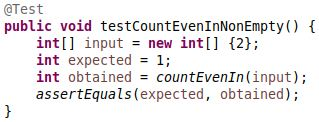
\includegraphics[width=.90\linewidth]{figures/stmtCoverageOrientedTests.JPG}
	\caption[Tests (cobertura de sentencias) para \emph{countEvenIn(int[])}]{Tests orientados a satisfacer cobertura de sentencias para el c\'odigo de \emph{countEvenIn(int[])} de la Figura~\ref{figures.code.coverageExample}.}
	\label{figures.examples.coverage.stmtTests}
\end{figure}

\begin{figure}
	\centering
	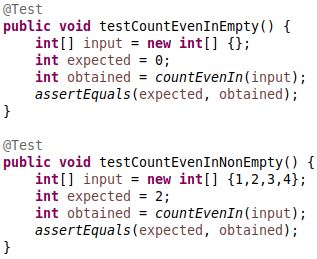
\includegraphics[width=.90\linewidth]{figures/branchCoverageOrientedTests.JPG}
	\caption[Tests (cobertura de ramas) para \emph{countEvenIn(int[])}]{Tests orientados a satisfacer cobertura de ramas para el c\'odigo de \emph{countEvenIn(int[])} de la Figura~\ref{figures.code.coverageExample}.}
	\label{figures.examples.coverage.branchTests}
\end{figure}

\begin{figure}
	\centering
	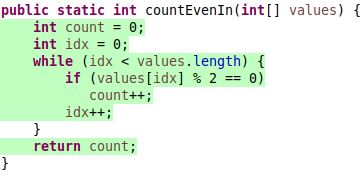
\includegraphics[width=.90\linewidth]{figures/branchCoverageExampleComplete.JPG}
	\caption[Cobertura de ramas del 100\% para \emph{countEvenIn(int[])}]{Medici\'on de cobertura de \emph{countEvenIn(int[])} de la Figura~\ref{figures.code.coverageExample} con una cobertura del 100\% tanto de sentencias como de ramas.}
	\label{figures.examples.coverage.fullCoverage}
\end{figure}

\begin{figure}
	\centering
	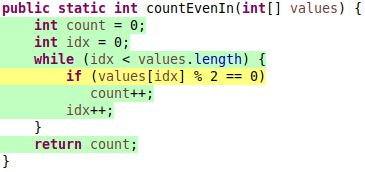
\includegraphics[width=.90\linewidth]{figures/branchCoverageExampleIncomplete.JPG}
	\caption[Cobertura de sentencias del 100\% para \emph{countEvenIn(int[])}]{Medici\'on de cobertura de \emph{countEvenIn(int[])} de la Figura~\ref{figures.code.coverageExample} con una cobertura del 100\% de sentencias pero no de ramas.}
	\label{figures.examples.coverage.stmtCoverage}
\end{figure}

En el caso de criterios de caja negra, varios criterios com\'unmente utilizados se basan en analizar la especificaci\'on de las entradas esperadas por el programa a analizar. En general se comienza partiendo el dominio de cada entrada de acuerdo a ciertas caracter\'isticas provistas. \'Estas deben dividir el conjunto de valores de cada entrada en subconjuntos disjuntos, y la uni\'on de todos los subconjuntos debe resultar en el dominio completo de cada entrada. Por ejemplo, si una entrada es un entero, es posible dar como caracter\'istica a \emph{ser par}, lo que divide todo el conjunto de los enteros en dos subconjuntos disjuntos (uno conteniendo todos los enteros pares y otro conteniendo a todos los impares), tal que al unir estos conjuntos se obtiene nuevamente a todos los enteros. Cada criterio basado en las entradas del programa a evaluar define de qu\'e forma combinar valores de cada subconjunto en los casos donde el programa tiene varias entradas. Por ejemplo, combinar todos con todos, o cada subconjunto debe estar representado por lo menos una vez sin importar con qu\'e otro subconjunto es combinado. Para el ejemplo de la Figura~\ref{figures.code.replaceExample}, que muestra un m\'etodo que dado un arreglo de enteros, un valor entero a buscar en el arreglo, y un valor con el cual reemplazar el valor anterior, realiza los reemplazos y retorna cuantos fueron realizados, en la Tabla \ref{tables.example.codeCoverage} se muestran posibles caracter\'isticas para dividir cada entrada: que el arreglo sea o no vac\'io; que el valor a buscar est\'e o no en el arreglo; y finalmente que el valor con el cual reemplazar al anterior sea igual o distinto al reemplazado. Vale aclarar que si bien todas las caracter\'isticas dividen las entradas en dos subconjuntos, esto no debe ser necesariamente as\'i. Una caracter\'istica que divida en m\'as subconjuntos es perfectamente v\'alida, siempre que cumpla con las propiedades mencionadas anteriormente. Como ejemplo de combinaci\'on de valores de cada subconjunto definidos por las caracter\'isticas en la Tabla \ref{tables.example.codeCoverage}, podemos utilizar el criterio \emph{Each Choice Value}, el cual determina que cada subconjunto debe estar representado al menos una vez en los tests. Esto lleva a los tests que se muestran en la Figura~\ref{figures.examples.coverage.eccTests}, donde tenemos dos tests, uno donde se utiliza un arreglo no vac\'io, con el valor a reemplazar perteneciendo al arreglo (2) y el valor con el cual reemplazar siendo igual al anterior; el segundo test utiliza un arreglo vac\'io, obviamente el elemento a buscar no pertenece al mismo y el valor con el cual se realiza el reemplazo es distinto al anterior. El hecho de que como se puede apreciar en la Figura~\ref{figures.examples.coverage.eccCoverage}, los tests anteriores logran una cobertura de ramas del 100\% al tiempo que \'estos son evidentemente un conjunto muy pobre de escenarios, sirve para remarcar c\'omo un criterio puede ser satisfecho al mismo tiempo que los tests que lo satisfacen son claramente de muy mala calidad.

\begin{figure}
	\lstinputlisting[basicstyle=\small, language=Java, tabsize=3]{results/draft/Replace.java}
	\caption[M\'etodo \emph{replace(int[], int, int)}]{M\'etodo para reemplazar todos los valores en un arreglo \emph{array} que son iguales a un valor especificado (\emph{what}) por otro valor especificado (\emph{with}) y retornar cuantos cambios se realizaron.}
	\label{figures.code.replaceExample}
\end{figure}

\begin{table}[]
	\caption[Caracter\'isticas para las entradas de \emph{replace(int[], int, int)}]{Caracter\'isticas con las que se puede dividir los conjuntos de las entradas del programa \emph{replace(int{[]}, int, int)} de la Figura~\ref{figures.code.replaceExample}.}
	\label{tables.example.codeCoverage}
	\centering
	\begin{tabular}{|c|ccc|}
		\hline
		Bloque & array vac\'io & what pertenece & with igual a what \\ \hline
		1 & T & T & T \\ \hline
		2 & F & F & F \\ \hline
	\end{tabular}
\end{table}

\begin{figure}
	\centering
	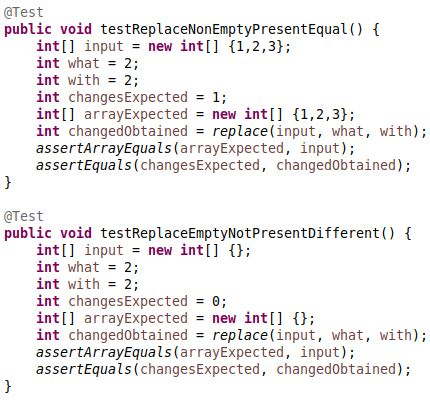
\includegraphics[width=.90\linewidth]{figures/replaceTestsEachChoice.JPG}
	\caption[Tests basados en \emph{ECC} para la Figura~\ref{figures.code.replaceExample} y las caracter\'isticas en la Tabla~\ref{tables.example.codeCoverage}]{Tests para satisfacer criterio de cobertura \emph{Each Choice Coverage} para \ref{figures.code.replaceExample} basado en las caracter\'isticas definidas en la Figura~\ref{tables.example.codeCoverage}.}
	\label{figures.examples.coverage.eccTests}
\end{figure}

\begin{figure}
	\centering
	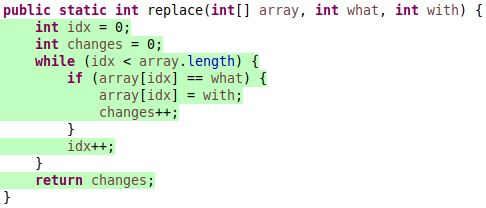
\includegraphics[width=\linewidth]{figures/replaceFullCoverage.JPG}
	\caption[Cobertura de ramas para los tests de la Figura~\ref{figures.examples.coverage.eccTests}]{Cobertura de ramas lograda por los tests definidos en la Figura~\ref{figures.examples.coverage.eccTests}.}
	\label{figures.examples.coverage.eccCoverage}
\end{figure}
